% ============================================================
% S2 导学件量产·批5 件1 —— 1.2.4 二面角（课时9 导学件）
% 轮4 成卷·S2 批5｜2026-09-12｜生成链：xelatex main.tex（两遍）→ python render.py（150dpi → png/pageN.png）
%
% 模板承 v11 样张族（经 课时02 首件／批1~批3 量产件）：六宏＝原样拷贝（L1 冻结参数零改动）；
%   课时页形制与局部宏（\pingtou/\liubai/\zhankong）照抄 课时06。
% 图＝源图位图（禁绘三维，公共规则§5）：figs/ 六件自 讲练件（上）定稿 docx word/media/ 原件解包
%   （restored351/image88/image116/image117/sub3_B_13/sub3_B_15，元素814/798/1138/1159/739/751，未改绘），
%   alt 缺失＝§四-5 照登。figs 与 docx 逐字节一致（解包原件）。
% 〔修图轮0913〕探究点一例1 配图换绘＝figPABCD_redraw0913.png（redraw351 退役不删，留存 figs/ 备查）：
%   装配本 p34 目验红旗——restored351（源书位图原件，元素814）题干不符：图内点集 C/A/M/B/A/D 缺顶点 P、
%   多题干外点 M、C 标注上残留坐标红字「(0.88,1.34,4.34)」，且彩色半透明面＋红箭头风格悖全书黑白线稿
%   （灰度印刷糊中灰）。本体＝两半平面二面角 GeoGebra 截图，点集拓扑与题干四棱锥 P-ABCD 不合（含双 A
%   标注），改标注不可达「与题干相符」，按修图令「重绘兜底」执行＝公共规则§5 三维禁重绘之用户逐件明示例外。
%   重绘＝精确坐标模型（AB∥CD，∠BAP=∠CDP=90°，PA=PD=AB=DC=1，∠APD=90°：A=(0,0,0) B=(1,0,0)
%   C=(1,√2,0) D=(0,√2,0) P=(0,√2/2,√2/2)），虚实线＝凸体面可见性判定（虚 CD/DA/PD，实 AB/BC/PA/PB/PC，
%   非手摆），cm 斜体标注，纯黑线白底零彩色（像素级断言 dev=0），图内零中文零记号。脚本＝
%   工作区/_tmp修图探点一课时09_0913/draw_fig.py；实证读数见修图轮回报（三零＋页数零变化＋600dpi 目验）。
%
% 取材链登记（盘点结论，详见 成卷/导学件/批5值台账.md）：
%   ① 讲练件（上）§1.2.4 讲部实态（dump_docx --slice 727:1254 取证＝工作区/_tmp批5S2量产0912/讲上-1.2.4全文.txt）：
%      知识讲解 条目 4 条（1.2.4-1 夹角〔含对比辨析表〕／-2 面积射影定理／-3 空间余弦定理／-4 空间正弦定理）＋
%      方法讲解（大招17 锐钝判定：直接观察／法向量内外分析／同等异补）＋题型例题 13 题（1.2.4.2.1-1～1.2.4.2.11-13）。
%   ② 探究点随讲部题型段主轴＝5 个：一 建系向量法·锐钝判定（1.2.4.2.1 段 -2 例／-1 变，同段双题入例变＝
%      批3 件1 口径）；二 等体积求距离与二面角（1.2.4.2.2 段 -3 例／变式命制）；三 射影面积法（1.2.4.2.7 段
%      -9 例／变式命制）；四 空间余弦定理（1.2.4.2.6 段 -8 例／变式命制）；五 折叠与夹角（1.2.4.2.8 段 -10 例／
%      变式命制）。池 -4/-5/-7/-11/-12/-13 六题未入本件（拓展册归置在册，登记备后轮）。
%   ③ 与课时09 练习轴 16 题互斥口径：课中探究同文件 池-2/-1 与练习轴第 4/3 题同文（题源＝讲部同号，
%      A-2「照用」计数互斥登记，同题双印不并计）；池-3/-9/-8/-10 未入练习轴。命制位＝判断 5＋变式 4（探究
%      二/三/四/五）＋评价 5＝14 题，与 16 题逐题零同文（题面/设问形态均异，断言见台账）。
%   ④ 课前预习 ZSD一/二/三＝讲部条目 1.2.4-1／-2／-3 同文化用（挖空值不印＝全品 p04 式）；
%      判断/评价＝恒命制位，逐题亲算登台账。1.2.4 无 v11 冻结导学件可回收＝回收 0。
%   ⑤ 记号/清稿性修复 2 处（非改题，登记）：池-2 题面「面PAD」→「平面PAD」（源件「平」字脱落类）；
%      池-3 题面两处内联【图】碎片按定稿C §4.4 复原为「直三棱柱ABC-A₁B₁C₁」「A₁C」。
%   ⑥ 句末标点：同文段承源「.」，新命制句用「．」（G8 成卷轮统一清扫，本件不单点改）。
% 编译门：三 0（error＝0／Overfull＝0／Missing character＝0，Underfull 仅计数）——读数见批5值台账。
% ============================================================
\documentclass[fontset=none]{ctexart}
\usepackage{qp-m3} % 换装：六宏→qp-m3 单包（钉后版 md5 7c3930362be8a0a2bdf21bbf8ac16573，两补钉随版）

% ================= 页脚参数宏（qp-headfoot 文件头明示的复用入口，非模块语义改动） =================
\renewcommand{\qpzhangming}{第一章\quad 空间向量与立体几何}
\renewcommand{\qpjianming}{导学件}
\renewcommand{\qpceming}{高中数学\quad 选择性必修第一册(人教B版)} % 换装回钉：qp-m3 默认册名＝选必二，防页脚漂移（试迁规约）

% ================= 局部宏（照抄 v11 导学增量/main.tex 冻结定义；不动公共模块） =================
% 局部宏 \pingtou 已由 qp-m3 收编（等值定义），依换装方案§1.4 预删防撞名
% 长度 \liubaoh 已由 qp-m3 分配，预删防重复定义
% 局部宏 \liubai 已由 qp-m3 收编（等值定义），依换装方案§1.4 预删防撞名
% 局部宏 \zhankong 已由 qp-m3 收编（等值定义），依换装方案§1.4 预删防撞名

% 纯题版孤行抑制（正装三裁①）：小结②操作/③收束独立段，pure 档整段隐藏，含详解版不受影响
\newcommand{\bindpx}[1]{\ifshowans\bindp{#1}\fi}

\begin{document}
%成书重装五本跨本连续页码（G7方案B，承M2/M3装配先例）setcounter 注入位
\setcounter{page}{36}

% ============================================================
% 课时页（第9课时；五段闭环）
% ============================================================
\keshi{第9课时\quad 二面角}
\mubiaoline
\mubiaomu{1}{理解二面角及其平面角的概念，会用定义法与射影面积法求二面角，记住二面角与两法向量夹角的关系；}
\mubiaomu{2}{掌握用空间向量求二面角（或两平面夹角）的建系坐标法，会用法向量夹角结合图形判定二面角的锐钝；}
\mubiaomu{3}{会用等体积法、空间余弦定理与翻折不变量求距离与角，体会几何问题代数化的转化思想.}

\vspace{1.7mm}
\begin{multicols}{2}
\emergencystretch=1em

% ---------- 课前预习（ZSD一/二/三＝讲部条目 1.2.4-1/-2/-3 同文化用） ----------
\huaxing{课}{前}{预}{习}{知识导学\quad 素养初识}

\zsd{一}{二面角及其平面角}

\tiaomu{1}{二面角：从一条直线出发的\kongbai{}所组成的图形叫做二面角，这条直线叫做二面角的\kongbai{}，每个半平面叫做二面角的面，记作二面角\(\alpha\text{-}l\text{-}\beta\)．\zhuzhu{类比平面角：以直线为「棱」、两个半平面为「面」；平面图形是两点一线，二面角是两「面」一线.}}

\tiaomu{2}{二面角的平面角：过二面角棱上\kongbai{}一点，分别在两个半平面内作\kongbai{}的两条射线，这两条射线所成的角叫做二面角的平面角；二面角的大小用它的平面角来度量，其范围为\kongbai{}．\zhuzhu{平面角的两边均与棱垂直，顶点在棱上；平面角的大小与顶点在棱上的位置无关.}}

\bindp \par\vspace{1.9mm}\penalty10000\noindent\makebox[\linewidth][c]{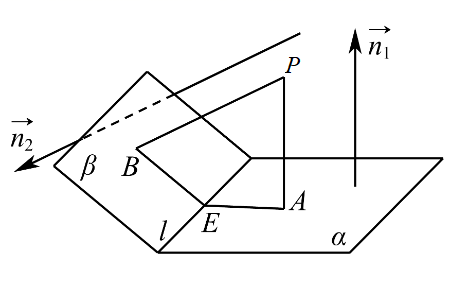
\includegraphics[width=40.0mm]{figs/sub3_B_13.png}}\par\vspace{-1.0mm}\penalty10000

\tiaomu{3}{向量法：若二面角\(\alpha\text{-}l\text{-}\beta\)的两个半平面的法向量分别为\(\overrightarrow{n_{1}}\)，\(\overrightarrow{n_{2}}\)，则\(|\cos\theta|=|\cos\langle\overrightarrow{n_{1}},\overrightarrow{n_{2}}\rangle|=\)\kongbai{}，而二面角\(\theta\)的大小与两法向量的夹角\kongbai{}或互补，须结合图形判定．\zhuzhu{「同负异正」：两法向量同指内侧（或同指外侧）时二面角与夹角互补，一内一外时相等.}}

\zhenhead{判断正误(正确的打\gou{},错误的打\cha{})}

\zhentib{(1)}{二面角的平面角的大小与顶点在棱上的位置有关．}

\begin{ansblock}[导-课时09-判1]
% ans:导-课时09-判1
\ansitem{(1)}{$\times$}
\end{ansblock}

\zhentib{(2)}{若两个半平面的法向量互相垂直，则这两个半平面构成的二面角的大小为\(90^{\circ}\)．}

\begin{ansblock}[导-课时09-判2]
% ans:导-课时09-判2
\ansitem{(2)}{\(\surd\)}
\end{ansblock}

\zsd{二}{面积射影定理}

\tiaomu{1}{面积射影定理：设平面图形的面积为\(S\)，它在平面\(\alpha\)内的射影图形的面积为\(S'\)，原图形所在平面与平面\(\alpha\)所成的二面角为\(\theta\)，则\(\cos\theta=\)\kongbai{}．\zhuzhu{二级结论：正投影后沿交线方向长度不变、垂直于交线方向的高变为原来的\(\cos\theta\)倍；解答题需先证后用.}}

\bindp \par\vspace{1.9mm}\penalty10000\noindent\makebox[\linewidth][c]{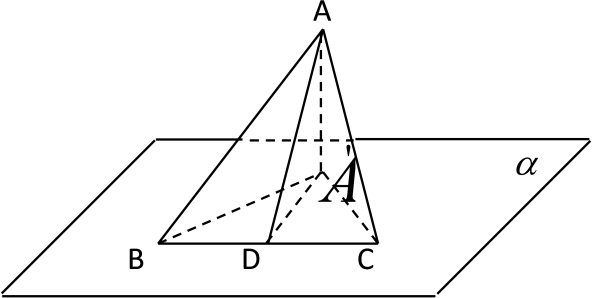
\includegraphics[width=48.0mm]{figs/sub3_B_15.png}}\par\vspace{-1.0mm}\penalty10000

\zhenhead{判断正误(正确的打\gou{},错误的打\cha{})}

\zhentib{(1)}{用射影面积法求二面角时，解答题中可直接引用结论，不必证明．}

\begin{ansblock}[导-课时09-判3]
% ans:导-课时09-判3
\ansitem{(1)}{$\times$}
\end{ansblock}

\zhentib{(2)}{平面图形在其射影平面内的射影图形的面积一定不大于原图形的面积．}

\begin{ansblock}[导-课时09-判4]
% ans:导-课时09-判4
\ansitem{(2)}{\(\surd\)}
\end{ansblock}

\zsd{三}{空间余弦定理}

\tiaomu{1}{空间余弦定理：在三面角\(O\text{-}ABC\)中，面角\(\alpha=\angle BOC\)，\(\beta=\angle COA\)，\(\gamma=\angle AOB\)，沿棱\(OC\)的二面角为\(C\)，则\(\cos C=\)\kongbai{}；特别地，当二面角\(C=90^{\circ}\)时，\(\cos\gamma=\)\kongbai{}．\zhuzhu{三面角中一面角与对面二面角互求的快算工具；解答题建议先证后用.}}

\begin{ansblock}[导-课时09-预习填空]
% ans:导-课时09-预习填空
\ansnote{预习填空}{知识点一：两个半平面；棱。知识点二：任一（棱上）；与棱垂直；\([0^{\circ},180^{\circ}]\)。知识点三：\(\dfrac{\overrightarrow{n_{1}}\cdot\overrightarrow{n_{2}}}{|\overrightarrow{n_{1}}||\overrightarrow{n_{2}}|}\)；相等；\(\dfrac{S^{\prime}}{S}\)；\(\dfrac{\cos\gamma-\cos\alpha\cos\beta}{\sin\alpha\sin\beta}\)；\(\cos\alpha\cos\beta\)。}
\end{ansblock}

\zhenhead{判断正误(正确的打\gou{},错误的打\cha{})}

\zhentib{(1)}{在三面角中，若棱\(OC\)处的二面角为直角，则\(\cos\gamma=\cos\alpha\cdot\cos\beta\)．}

\begin{ansblock}[导-课时09-判5]
% ans:导-课时09-判5
\ansitem{(1)}{\(\surd\)}
\end{ansblock}

\liubai[9mm]{此处书写}

% ---------- 课中探究（探究点5个＝讲部题型段主轴；例1/变式1同文位＝讲部题面逐字(记号LaTeX化)；素养小结＝讲部题型通式编注化用） ----------
\huaxing{课}{中}{探}{究}{考点探究\quad 素养小结}

\tjdnr{一}{建系向量法求二面角(锐钝判定)}{例\textbf{1}}{中档(知识点一)}{如图，在四棱锥\(P\text{-}ABCD\)中，\(AB\parallel CD\)，且\(\angle BAP=\angle CDP=90^{\circ}\)．(1)证明：平面\(PAB\perp\)平面\(PAD\)；(2)若\(PA=PD=AB=DC\)，\(\angle APD=90^{\circ}\)，求二面角\(A\text{-}PB\text{-}C\)的余弦值.}

\bindp \par\vspace{1.9mm}\penalty10000\noindent\makebox[\linewidth][c]{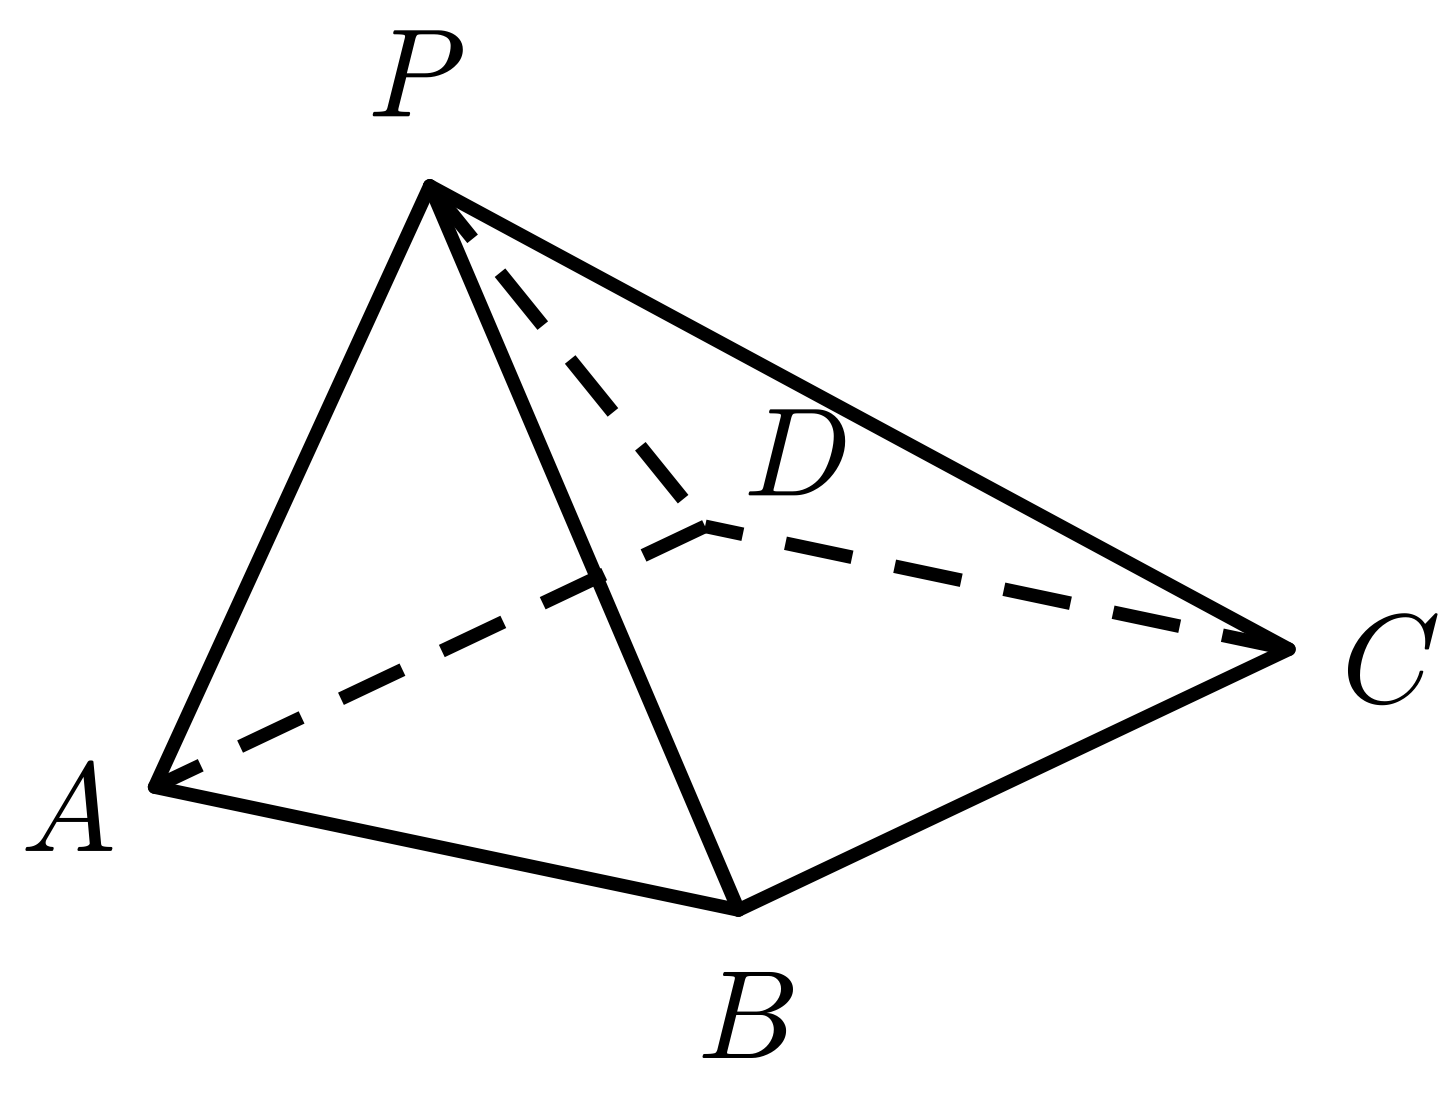
\includegraphics[width=40.0mm]{figs/figPABCD_redraw0913.png}}\par\vspace{-1.0mm}\penalty10000

\liubai[12mm]{解答书写区}

\begin{ansblock}[导-课时09-探1-例1]
% ans:导-课时09-探1-例1
\ansnote{例1}{\(-\dfrac{\sqrt{3}}{3}\)}
\ansnote{解析}{\(\angle APD=90^{\circ}\)（\(\angle ADP=45^{\circ}\)，故 \(PD\perp PA\)）。}
\ansnote{解析}{求的是平面 \(FAD\) 与平面 \(ADC\) 的夹角。}
\end{ansblock}

\liB{变式\textbf{1}}{中档(知识点一)}{}{如图所示的几何体中，\(BE\perp BC\)，\(EA\perp AC\)，\(BC=2\)，\(AC=2\sqrt{2}\)，\(\angle ACB=45^{\circ}\)，\(AD\parallel BC\)，\(BC=2AD\)．(1)求证：\(AE\perp\)平面\(ABCD\)；(2)若\(\angle ABE=60^{\circ}\)，点\(F\)在\(EC\)上，且满足\(EF=2FC\)，求平面\(FAD\)与平面\(ADC\)的夹角的余弦值.}

\bindp \par\vspace{1.9mm}\penalty10000\noindent\makebox[\linewidth][c]{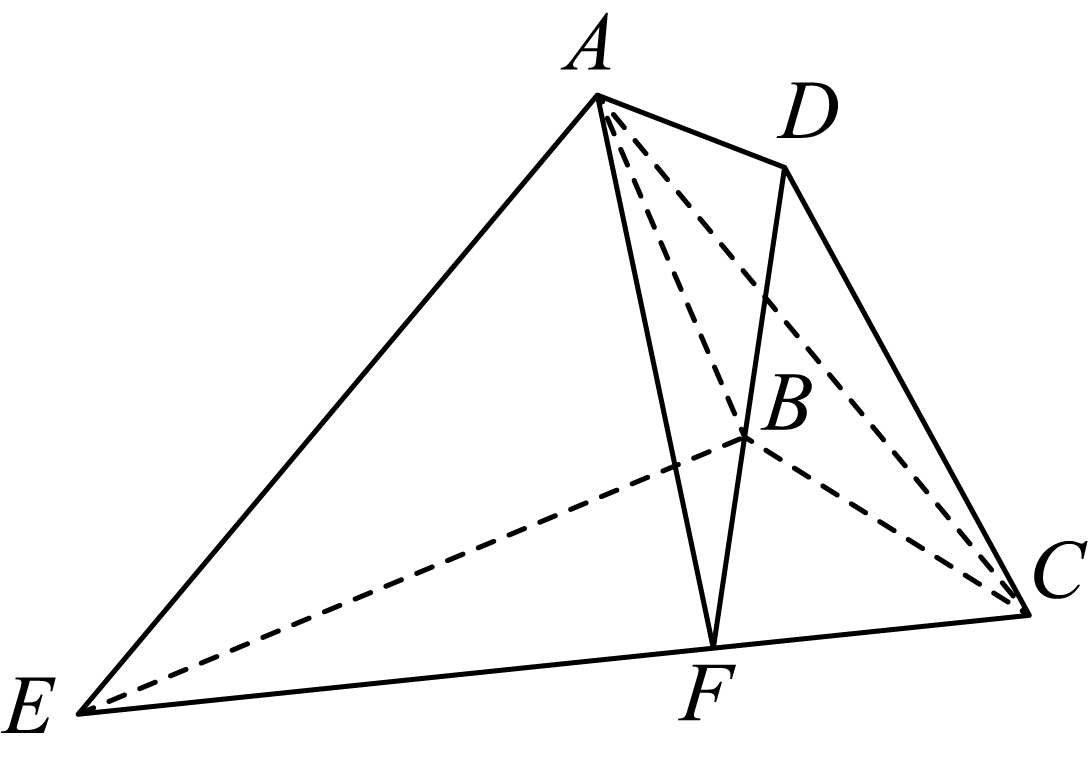
\includegraphics[width=38.0mm]{figs/image88.png}}\par\vspace{-1.0mm}\penalty10000

\liubai[8mm]{解答书写区}

\begin{ansblock}[导-课时09-探1-变式1]
% ans:导-课时09-探1-变式1
\ansnote{变式1}{\(\dfrac{2\sqrt{7}}{7}\)}
\end{ansblock}

\xiaojie{①识别：题干要求证明垂直并求二面角(或两平面夹角)的余弦值时，判归本题型.}

\bindpx {\kaishu ②操作：先完成垂直证明，确定可建系的两两垂直的三条直线；建系写出相关点坐标，求两个半平面的法向量并算数量积.}

\bindpx {\kaishu ③收束：按图形判定二面角是锐角还是钝角定符号——两法向量同指内侧(或同指外侧)时二面角与法向量夹角互补(同负异正)，一内一外时相等；求平面夹角则直接取绝对值.}

\tjdnr{二}{等体积求距离与二面角}{例\textbf{1}}{中档(知识点一)}{如图，直三棱柱\(ABC\text{-}A_{1}B_{1}C_{1}\)的体积为4，\(\triangle A_{1}BC\)的面积为\(2\sqrt{2}\)．(1)求\(A\)到平面\(A_{1}BC\)的距离；(2)设\(D\)为\(A_{1}C\)的中点，\(AA_{1}=AB\)，平面\(A_{1}BC\perp\)平面\(ABB_{1}A_{1}\)，求二面角\(A\text{-}BD\text{-}C\)的正弦值.}

\liubai[12mm]{解答书写区}

\begin{ansblock}[导-课时09-探2-例1]
% ans:导-课时09-探2-例1
\ansnote{例1}{(1)\(\sqrt{2}\)；(2)\(\dfrac{\sqrt{3}}{2}\)}
\ansnote{解析}{方程组法独立可解（叉乘法从略）。}
\end{ansblock}

\liB{变式\textbf{1}}{简单(知识点一)}{}{已知三棱锥\(P\text{-}ABC\)中，\(PA\perp\)平面\(ABC\)，\(AB\perp BC\)，\(AB=BC=2\)，\(PA=3\)，则点\(A\)到平面\(PBC\)的距离为\kongbai{}．}

\begin{ansblock}[导-课时09-探2-变式1]
% ans:导-课时09-探2-变式1
\ansnote{变式1}{\(\dfrac{6\sqrt{13}}{13}\)}
\end{ansblock}

\xiaojie{①识别：题干第(1)问求点到平面的距离、第(2)问求二面角且两问共用垂直关系时，判归本题型.}

\bindpx {\kaishu ②操作：第一步用等体积法换底求点面距离；再由距离反推棱长并确定两两垂直的三条棱建系.}

\bindpx {\kaishu ③收束：求两平面法向量算余弦，按所问取正弦或余弦；换底时底与高须对应.}

\tjdnr{三}{射影面积法求二面角}{例\textbf{1}}{中档(知识点二)}{如图，\(\triangle ABC\)与\(\triangle BCD\)所在平面垂直，且\(AB=BC=BD\)，\(\angle ABC=\angle DBC=120^{\circ}\)，则二面角\(A\text{-}BD\text{-}C\)的余弦值为\kongbai{}.}

\bindp \par\vspace{1.9mm}\penalty10000\noindent\makebox[\linewidth][c]{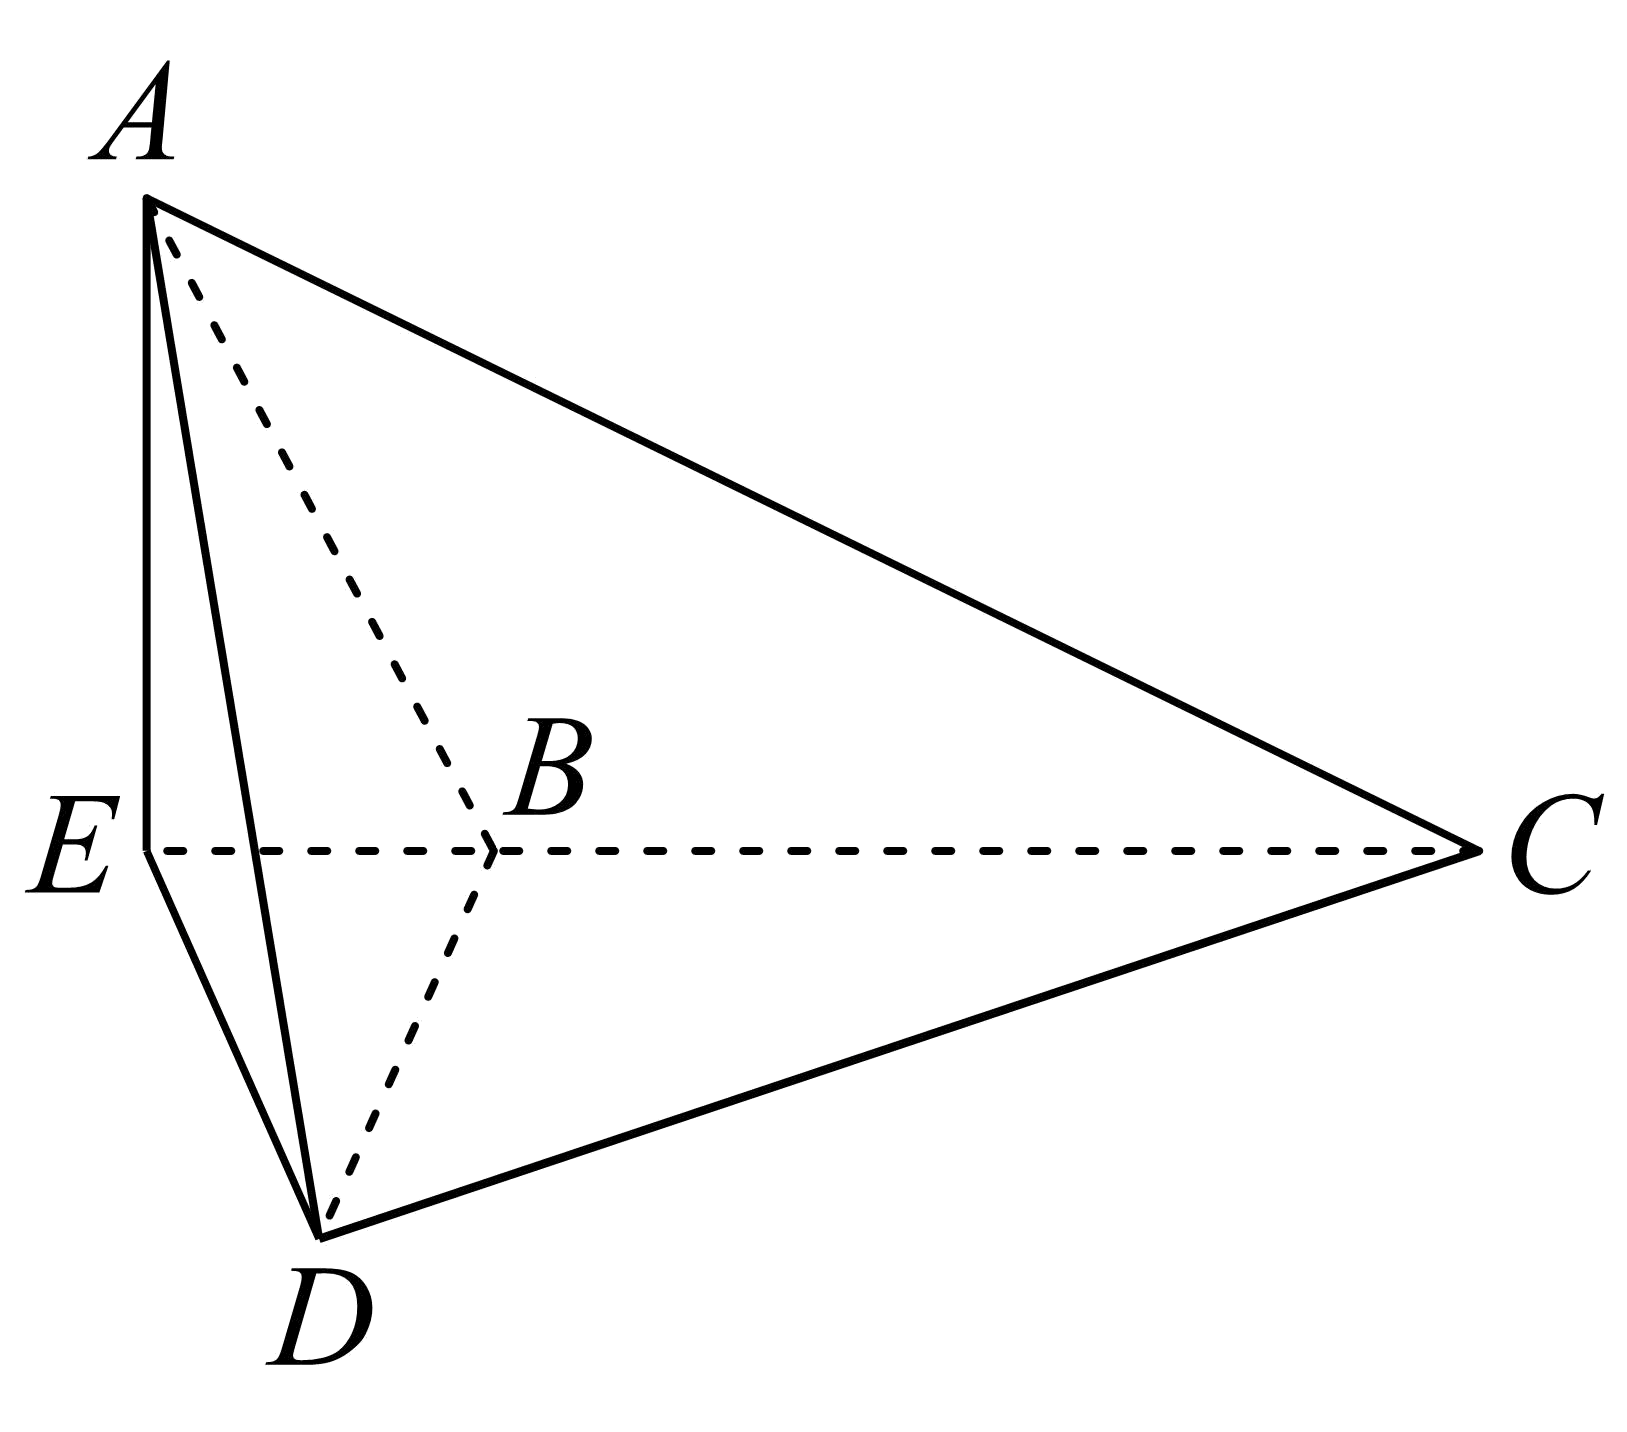
\includegraphics[width=36.0mm]{figs/image116.png}}\par\vspace{-1.0mm}\penalty10000

\liubai[8mm]{解答书写区}

\begin{ansblock}[导-课时09-探3-例1]
% ans:导-课时09-探3-例1
\ansnote{例1}{\(-\dfrac{\sqrt{5}}{5}\)}
\end{ansblock}

\liB{变式\textbf{1}}{中档(知识点二)}{}{二面角\(\alpha\text{-}l\text{-}\beta\)中，\(\triangle ABC\)在半平面\(\alpha\)内，\(A\)，\(B\)在棱\(l\)上，且\(\triangle ABC\)的面积为2，\(\triangle ABC\)在半平面\(\beta\)内的射影三角形的面积为1。若二面角\(\alpha\text{-}l\text{-}\beta\)为钝二面角，则其大小为\kongbai{}．}

\begin{ansblock}[导-课时09-探3-变式1]
% ans:导-课时09-探3-变式1
\ansnote{变式1}{\(120^{\circ}\)}
\end{ansblock}

\xiaojie{①识别：无棱二面角或平面角作图困难、两个面内三角形的面积易求时，判归本题型.}

\bindpx {\kaishu ②操作：先由面面垂直找出一个面内三角形在另一个面内的射影三角形，分别计算原三角形与射影三角形的面积.}

\bindpx {\kaishu ③收束：由\(\cos\theta=S_{\text{射}}/S_{\text{原}}\)求出夹角余弦，再核对所求二面角与该夹角是否互补以定符号.}

\tjdnr{四}{空间余弦定理求二面角}{例\textbf{1}}{中档(知识点三)}{\(AB\)是圆的直径，\(PA\)垂直于圆所在的平面，\(C\)是圆上的点，平面\(PAC\perp\)平面\(PBC\)，若\(AB=2\)，\(AC=1\)，\(PA=1\)，求二面角\(C\text{-}PB\text{-}A\)的余弦值.}

\liubai[10mm]{解答书写区}

\begin{ansblock}[导-课时09-探4-例1]
% ans:导-课时09-探4-例1
\ansnote{例1}{\(\dfrac{\sqrt{6}}{4}\)}
\ansnote{解析}{空间余弦定理先证后用（建系可另证）。}
\end{ansblock}

\liB{变式\textbf{1}}{简单(知识点三)}{}{在三面角\(O\text{-}ABC\)中，面角\(\alpha=\angle BOC=60^{\circ}\)，\(\beta=\angle COA=45^{\circ}\)，且沿棱\(OC\)的二面角\(C\)为直角，则\(\cos\gamma=\cos\angle AOB=\)\kongbai{}．}

\begin{ansblock}[导-课时09-探4-变式1]
% ans:导-课时09-探4-变式1
\ansnote{变式1}{\(\dfrac{\sqrt{2}}{4}\)}
\end{ansblock}

\xiaojie{①识别：所求二面角的棱恰为某三面角的棱、且三个面角容易求出时，判归本题型.}

\bindpx {\kaishu ②操作：由直径、线面垂直等条件求出三面角三条棱方向的三个面角(余弦)，认准所求二面角对应三面角的哪条棱.}

\bindpx {\kaishu ③收束：代入空间余弦定理\(\cos C=\frac{\cos\gamma-\cos\alpha\cos\beta}{\sin\alpha\sin\beta}\)计算；当二面角为直角时退化为\(\cos\gamma=\cos\alpha\cos\beta\).}

\tjdnr{五}{折叠与两平面夹角}{例\textbf{1}}{中档(知识点二)}{如图(1)，在直角梯形\(ABCD\)中，\(AB\parallel CD\)，\(AB\perp BC\)，且\(BC=CD=\frac{1}{2}AB=2\)，取\(AB\)的中点\(O\)，连结\(OD\)，并将\(\triangle AOD\)沿着\(OD\)翻折，翻折后\(AC=2\sqrt{3}\)，点\(M\)，\(N\)分别是线段\(AD\)，\(AB\)的中点，如图(2)．(1)求证：\(AC\perp OM\)；(2)求平面\(OMN\)与平面\(OBCD\)夹角的余弦值.}

\bindp \par\vspace{1.9mm}\penalty10000\noindent\makebox[\linewidth][c]{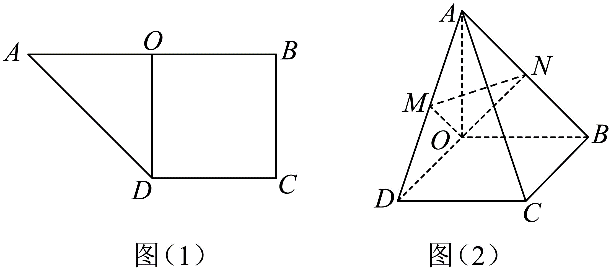
\includegraphics[width=55.0mm]{figs/image117.png}}\par\vspace{-1.0mm}\penalty10000

\liubai[8mm]{解答书写区}

\begin{ansblock}[导-课时09-探5-例1]
% ans:导-课时09-探5-例1
\ansnote{例1}{\(\dfrac{\sqrt{3}}{3}\)}
\end{ansblock}

\liB{变式\textbf{1}}{简单(知识点一)}{}{将边长为\(2\sqrt{3}\)的正三角形\(ABC\)沿高线\(AD\)折成直二面角\(B\text{-}AD\text{-}C\)，则折后\(B\)，\(C\)两点间的距离为\kongbai{}．}

\begin{ansblock}[导-课时09-探5-变式1]
% ans:导-课时09-探5-变式1
\ansnote{变式1}{\(\sqrt{6}\)}
\end{ansblock}

\xiaojie{①识别：平面图形翻折后求两平面的夹角(二面角)或翻折后线段长时，判归本题型.}

\bindpx {\kaishu ②操作：用翻折前后的不变量(长度、垂直)与新增条件(如翻折后某线段长)锁定折后结构，常先证线面垂直.}

\bindpx {\kaishu ③收束：选射影面积比或建系求法向量两种路径之一；求平面夹角时余弦取绝对值.}

% ---------- 课堂评价（恒 5 题＝3 单选＋2 填空；4 简单＋1 中档≤例题；提示词形制；全命制——逐题亲算登批5值台账） ----------
\begin{ketang}{本组共5题，1—3为单选，4—5为填空．}

\jiancestem{{\fontsize{11.4pt}{14pt}\selectfont\heihao {\numboldjian 1}．}\hspace{4.1mm}\tieside{简单(知识点一)}\hspace{2.2mm}下列关于二面角的说法中，正确的是(\kongwei)}

\bindopt {\fontsize{10.5pt}{21pt}\selectfont A．二面角的大小范围是\((0^{\circ},90^{\circ}]\)；\par}

\bindopt {\fontsize{10.5pt}{21pt}\selectfont B．二面角的平面角的两条边都与棱垂直\par}

\bindopt {\fontsize{10.5pt}{21pt}\selectfont C．任意两个相交平面构成的四个二面角的大小都相等；\par}

\bindopt {\fontsize{10.5pt}{21pt}\selectfont D．二面角的大小等于其两个半平面的法向量的夹角\par}

\begin{ansblock}[导-课时09-评1]
% ans:导-课时09-评1
\ansitem{1}{B}
\end{ansblock}

\jiancestem{{\fontsize{11.4pt}{14pt}\selectfont\heihao {\numboldjian 2}．}\hspace{4.1mm}\tieside{简单(知识点一)}\hspace{2.2mm}已知二面角\(\alpha\text{-}l\text{-}\beta\)的大小为\(120^{\circ}\)，其两个半平面的法向量分别为\(\overrightarrow{n_{1}}\)，\(\overrightarrow{n_{2}}\)，则\(\langle\overrightarrow{n_{1}},\overrightarrow{n_{2}}\rangle\)的大小为(\kongwei)}

\bindopt {\fontsize{10.5pt}{21pt}\selectfont \makebox[\dimexpr0.5\linewidth-1em\relax][l]{A．\(30^{\circ}\)；}\makebox[\dimexpr0.5\linewidth-1em\relax][l]{B．\(60^{\circ}\)；}\par}

\bindopt {\fontsize{10.5pt}{21pt}\selectfont \makebox[\dimexpr0.5\linewidth-1em\relax][l]{C．\(60^{\circ}\)或\(120^{\circ}\)；}\makebox[\dimexpr0.5\linewidth-1em\relax][l]{D．\(150^{\circ}\)}\par}

\begin{ansblock}[导-课时09-评2]
% ans:导-课时09-评2
\ansitem{2}{C}
\end{ansblock}

\jiancestem{{\fontsize{11.4pt}{14pt}\selectfont\heihao {\numboldjian 3}．}\hspace{4.1mm}\tieside{简单(知识点二)}\hspace{2.2mm}已知一个平面图形的面积为\(2\sqrt{3}\)，它在平面\(\alpha\)内的射影图形的面积为\(\sqrt{3}\)，则该图形所在平面与平面\(\alpha\)所成二面角的余弦值为(\kongwei)}

\bindopt {\fontsize{10.5pt}{21pt}\selectfont \makebox[\dimexpr0.25\linewidth-0.5em\relax][l]{A．\(\frac{1}{2}\)；}\makebox[\dimexpr0.25\linewidth-0.5em\relax][l]{B．\(\frac{\sqrt{3}}{2}\)；}\makebox[\dimexpr0.25\linewidth-0.5em\relax][l]{C．\(\frac{\sqrt{2}}{2}\)；}\makebox[\dimexpr0.25\linewidth-0.5em\relax][l]{D．\(\frac{1}{3}\)}\par}

\begin{ansblock}[导-课时09-评3]
% ans:导-课时09-评3
\ansitem{3}{A}
\end{ansblock}

\jiancestem{{\fontsize{11.4pt}{14pt}\selectfont\heihao {\numboldjian 4}．}\hspace{4.1mm}\tieside{简单(知识点一)}\hspace{2.2mm}已知二面角\(\alpha\text{-}l\text{-}\beta\)的大小为\(60^{\circ}\)，\(A\in\alpha\)，\(B\in\beta\)，\(AP\perp l\)，\(BP\perp l\)，垂足均为\(P\)，且\(PA=PB=1\)，则\(AB=\)\kongbai{}．{\zhushi{(提示：\(AP\)、\(BP\)均垂直于棱，故\(\angle APB\)是二面角的平面角；再用等边三角形的判定或余弦定理)}}}

\begin{ansblock}[导-课时09-评4]
% ans:导-课时09-评4
\ansitem{4}{1}
\end{ansblock}

\jiancestem{{\fontsize{11.4pt}{14pt}\selectfont\heihao {\numboldjian 5}．}\hspace{4.1mm}\tieside{中档(知识点三)}\hspace{2.2mm}在三面角\(O\text{-}ABC\)中，面角\(\alpha=\angle BOC=60^{\circ}\)，\(\beta=\angle COA=90^{\circ}\)，\(\gamma=\angle AOB=60^{\circ}\)，则沿棱\(OC\)的二面角\(C\)的余弦值为\kongbai{}．{\zhushi{(提示：直接代入空间余弦定理\(\cos C=\frac{\cos\gamma-\cos\alpha\cos\beta}{\sin\alpha\sin\beta}\)，注意\(\beta=90^{\circ}\)时\(\cos\beta=0\))}}}

\begin{ansblock}[导-课时09-评5]
% ans:导-课时09-评5
\ansitem{5}{\(\dfrac{\sqrt{3}}{3}\)}
\end{ansblock}

\end{ketang}

\end{multicols}

\tailfill
\end{document}
